
%% ==============
\chapter{Installationsunterst�tzung in Smart-Environments}
\label{ch:Arbeiten}
%% ==============

Als erstes wird eine Studie zur Installation von Heimautomatisierungssystemen
und deren Einsichten in den Installationsprozess der Anwender vorgestellt. Dabei
werden .. Darauf folgend wird ein Ansatz pr�sentiert der eine Messung des
Installationsfortschrittes verwendet, um aktive Unterst�tzung w�hrend des
Prozesses zu leisten. Einflussfaktoren auf die bei einer Installation auftreten
k�nnen werden auch diskutiert.[bleargh..]


%% ==============
\section{Sensorinstallation f�r Ubicomp-Systeme in Heimumgebungen}
\label{sec:assemblyRequired}
%% ==============

% =======
\subsection{Eigenschaften einer Sensorinstallation}
% =======

Die Installation von Sensoren wird in \cite{Beckmann2004} als eine Aufgabe mit
zwei Dimensionen betrachtet: Platzierung und Assoziation.
Die Platzierung ist wichtig um den Sensorknoten zu erlauben die korrekte
physikalische Gr��e mit ausreichender Qualit�t zu messen. Die Positionierung
wird weiterhin in zwei Unterfaktoren aufgeteilt: \emph{Direktionalit�t} und
\emph{Proximit�t}.
Unter dem Direktionalit�tsfaktor versteht man wie sensibel der Sensor auf
Fehlern in seiner Ausrichtung reagiert. Eine Kamera ist zum Beispiel sehr darauf
angewiesen, dass sie die richtige Szene aufnimmt, ein Mikrofon hingegen ist
nicht so sensibel auf seine Ausrichtung. Der Proximit�tsfaktor gibt an wie nahe
der Sensor an sein Messziel angebracht werden muss.
Die Assoziation bezieht sich auf die semantische verbindung zwischen dem
Datenstrom eines Sensors und des gemessenen Objektes in der realen Welt. Eine
Eins-zu-Eins Assoziation ist f�r Menschen die einfachste Variante und kann viel
leichter nachvollzogen werden. Die Pr�zision einer Assoziation wird als Funktion
der KnotenPlazierung und dessen zu messenden Subjekts beschrieben.
Es wird betont, dass die Assoziation eines proximit�ts Sensors leichter
durchzuf�hren ist als die eines direktionalen Sensors. Au�erdem ist auch das
Beobachten von Objekten leichter als das Monitoring von R�umen weil die
Reichtweite eines Sensors schwer einzugrenzen ist.

% =======
\subsection{Ablauf der Studie}
% =======

Die Studie wurde in 15 Haushalten aus den Vereinigten Staaten
durchgef�hrt. Die Teilnehmer wurden als repr�sentative Gruppe von
einer Marktforschungsfirma ausgesucht und es wurde darauf geachtet,
dass sich keine Experten unter den Teilnehmern befinden sollen. Als
Entlohnung bekamen die Teilnehmer eine Geldsumme. Die Daten der
Installationsdurchf�hrung, die im Durchschnitt etwa 84 Minuten
gedauert hat, wurden von zwei Mitarbeitern gesammelt. Diese haben mit
Hilfe von Notizen und Fotos jeden Installationsversuch dokumentiert.
Ein Fragebogen wurde von jedem Teilnehmer ausgef�llt.

Der Ablauf einer Installation hatte vier Phasen: \emph{Einleitung,
Erkundung, Installation der Sensoren und ein Interview}.
In der Einleitung wurde eine Freigabeform und ein Fragebogen
ausgeteilt (die Inhalte dieser Dokumente wurde nicht publiziert). Die
Erkundungsphase diente um eine �bersicht des Konzepts hinter dem
Ubicomp-System und dem Installationskit zu geben. In der
Installationsphase wurden die Teilnehmer gebeten jeden der
mitgelieferten Sensoren einzeln an ein Ger�t oder in einem Raum
aufzustellen. Die Evaluatoren haben w�hrend der Installationphase
keine Fragen mehr �ber den Prozess beantwortet und haben versucht kein
Feedback �ber die Handlungen der Teilnehmer zu geben um die
Resultate der Studie nicht zu verf�lschen.

Nach der Installationsphase wurde ein Interview durchgef�hrt. Die
Fragen dienten dazu das Verstehen der Teilnehmer �ber die
verschiedenen Installationsschritte und Komponenten des Systems zu
erfassen und um die Probleme zu identifizieren w�rde das System einen
Monat lang angebracht bleiben. Es wurde auch gefragt wie sie die
Sensoren davon abbringen w�rden Daten zu sammeln.

% =======
\subsection{Aufbau des Kits}
% =======

Das Kit wurde so konzipiert, dass die Installation keine komplexen Schritte, wie
�nderungen an dem elektrischen Sicherungskasten, enth�lt. Der
Inhalt des Kits ist wie folgender gewesen (siehe auch Abbildung
\ref{fig:assembly-kit}):
\begin{itemize}
  \item Mock-Up-Sensoren (Vibration, Strom, Bild, Ger�usch)
  \item Ein Katalog mit Gegenst�nden 
  \item Ein kompakter Computer
  \item PDA Ger�t f�r Barcodes
  \item Anweisungen der Version A,B und C (vgl. Tabelle \ref{tab:assembly_doku})
\end{itemize}

Ein Teil der mitgelieferten Sensoren wurden konzipiert um die
Aktivit�t von Haushaltsger�ten zu messen (Vibration, Strom,
Ger�usche). Bewegungssensoren und Kameras wurden benutzt um die
Aktivit�t der Menschen und das elektrische Licht zu �berwachen.
Die Sensoren wurden je nach Typ Farbkodiert und es wurden nur 2
Sensoren von jedem Typ, insgesamt 10, mitgeliefert. In Realit�t w�rde
eine solche Ubicomp-Anwendung mehr als 50 Sensoren beinhalten. Nur die
Platiezunrung und Assoziation der Sensoren wurde in betracht genommen.
Zusammenarbeit oder Korrelation der Sensoren wurde nicht betrachtet,
daher konnte die Installation jedes einzelnen Sensors unabh�ngig
betrachtet werden.

\begin{figure}[htb]
  \centering
  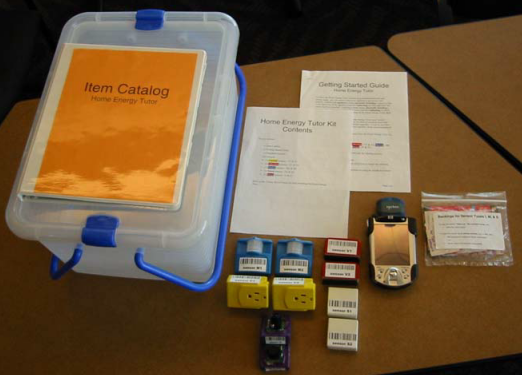
\includegraphics[width=0.8\textwidth]{img/assembly-kit.png}
  \caption{Bild des Kits}
  \label{fig:assembly-kit}
\end{figure}

Der Katalog mit Gegenst�nden enthielt Barcodes f�r alle m�glichen
Ger�tetypen die in einem Haushalt auftreten k�nnen, wie z.B.
K�hlschr�nke oder Waschmaschienen. Dieser Katalog in Zusammenhang mit
den Barcodes auf den Sensoren und dem Barcodereader wurden benutzt um
die Assoziation zwischen den Sensoren und ihren Subjekten
durchzuf�hren. Der kompakte Computer sollte Daten von den
Wireless-Sensoren auslesen. Die einzige Interaktion die der Nutzer mit
dem Computer hatte war es ihn mit Strom zu versorgen.\\
Ein Scanner und gedruckte Anweisungen wurden den Nutzern �berreicht um
sie durch den Installationsprozess zu f�hren. Es wurden verschiedene
Anweisungen ausgeteilt um zu vermeiden, dass die Studie die Qualit�t
der Nutzeranleitung bewertet. Das Ziel der Studie war es die
Sensorinstallation zu betrachten. In Tabelle \ref{tab:assembly_doku}
werden die Unterschiede zwischen den Dokumentationstypen aufgezeigt.
Die Namen der Sensoren in Dokumentation A und B waren gleich
(\emph{Strom, Vibration, Bewegung, Bild, Ger�usch}). In version C der
Dokumentation wurden nur Farben benutzt um zwischen den Sensoren zu
unterscheiden. Alle Sensoren mussten mit Hilfe des PDAs assoziiert
werden in dem der Sensor und das zu messende Objekt aus dem Katalog
eingescannt wurden. Eine richtige Installation wurde nach den
Positionierungs- und Assoziationsfaktoren bewertet. Es wird erw�hnt,
dass es keine statistisch signifikanten Unterschiede, zwischen dem
Erfolg der Installation im Zusammenhang mit den verschiedenen
Dokumentationen, gab. Von den 5 Nutzern mit Dokumentation C
haben sich 3 solche Informationen aber gew�nscht.

\begin{table}
  \caption{Die Unterschiede zwischen den Dokumentationen}
  \centering
  \begin{tabular}{l c c c}
    %heading
    \hline\hline  
    Enthaltene Informationen & Dokumentation A & Dokumentation B &
    Dokumentation C  \\ [1ex]
    \hline
    %heading end
	Installationsanleitung & \checkmark & \checkmark & \checkmark \\
	[1ex] 
	Gesammelte Daten & \checkmark & \checkmark & x \\ [1ex]
	Funktion der Sensoren & \checkmark & x & x \\ [1ex] 
    \hline
  \end{tabular}
  \label{tab:assembly_doku}
\end{table}

% =======
\subsection{Resultate der Studie}
% =======

Die Resultate der Evaluierung werden im Folgenden
zusammengefasst.

Von den 150 Sensorinstallationsaufgaben (15 Teilnehmer x 10 Sensoren)
wurden 112 (75\%) erfolgreich durchgef�hrt. Nur 5 Teilnehmer (30\%)
haben alle Aufgaben korrekt durchgef�hrt. Das Einlesen mit dem
Barcode-Scanner wurde von 13 aus 15 (86\%) Teilnehmern korrekt
durchgef�hrt. Zwei der f�nfzehn Teilnehmer konnten keine der Aufgaben
erf�llen und haben auch die Assoziation mit Hilfe des Barcodes nicht
verstanden. Dieselben konnten weder den Anweisungen auf dem PDA
folgen, noch wussten sie wie die Sensoren zu deaktivieren sind. Nur 5
aus den 10 Teilnehmern, die Beschreibungen der von den Sensoren
aufgenommenen Daten erhalten haben (Dokumentation A und B), konnten
den konkreten Anwendugsfall der Sensoren nennen. Der am meisten
fehlerhaft installierte Sensor war der Ger�uschsensor, mit 67\%
Erfolgsrate, gefolgt von dem Bildsensor, mit 70\% Erfolgsrate. Im
Vergleich dazu wurde der Stromsensor (ein Steckdosenaufsatz) in 87\%
der F�lle erfolgreich installiert (korrekte Assoziation 87\% und
korrekte Platzierung 93\%). 8 von den 15 Teilnehmern (53\%) haben
wenigstens einen, aber nicht alle Sensoren korrekt installiert.
Vier der neun fehlerhaften Bildsensorinstallationen folgten aus dem
�bersehen oder nicht folgen der Ausrichtungsanweisungen.
Mit Hilfe der Information �ber die Sensoren konnte ein Nutzer einen
Sensor erfolgreich an seinen nicht standardkonformen K�hlschrank
anbringen.

Obwohl vor der Studie alle Teilnehmer �ber die Datenerfassung
unterrichtet wurden und der Aspekt, dass die Daten das Haus nicht
verlassen mehrmals erw�hnt wurde, gab es zwei Teilnehmer die sich
geweigert haben die Bildsensoren zu installieren. Andere Teilnehmer
hatten sich auch mit Bedenken �ber die Erfassung der Daten ge�u�ert.
Die Teilnehmer hatten auch Bedenken dass die Installation ihren
Einrichtungen schaden w�rden und, dass Haustiere oder Kinder an die
Sensoren kommen k�nnten.


% =======
\subsection{Design Prinzipien}
% =======

Im folgenden werden die 5 in \cite{Beckmann2004} erhobenen
Design-Prinzipien f�r die Endnutzerinstallation von Sensoren
aufgef�hrt und erl�utert. Die ersten zwei Prinzipien lehnen sich an
traditionelle Prinzipien aus der Mensch-Maschine-Interaktion. Die
letzten drei sind Erkenntnisse die aus der Studie gewonnen wurden.
\begin{enumerate}
  \item \textbf{Das Konzeptuelle Modell des Benutzer bei bekannten
  Technologien angemessen nutzen}\\ Sensortypen deren Funktionalit�t
  �hnlich ist wie in anderen Anwendungsszenarien k�nnen die Benutzer
  beim Verst�ndnis unterst�tzen, da die Konzeptuellen Modelle der
  Nutzer nicht mehr redefiniert werden m�ssen. Man muss aber darauf
  achten, dass vertraute Technologie nicht anders angewendet wird als
  im Normalfall. Falls dies dennoch auftritt, kann der Sensor sowohl
  im Namen als auch im Aussehen versteckt werden.
  \item \textbf{Nutzbarkeit der Installation mit den h�uslichen
  Anliegen im Gleichgewicht halten} \\
  Designer und Anwender m�ssen Faktoren der �sthetik und der Umgebung
  unter Betracht nehmen. Wenn Benutzer aus pragmatischen Gr�nden die
  Installation nicht durchf�hren wollen, k�nnen Technische Aspekte
  leicht in den Hintergrund treten. Ein System, dass die
  Privatsph�re oder das Eigentum des Besitzers verletzt kann genauso
  in der Box liegen gelassen werden wie ein System, das schwer zu
  installieren ist.
  \item \textbf{Die Anwendung von Kameras, Mikrophonen und
  hochdirektionalen Sensoren vermeiden}\\
  Nicht nur die Sensitiven Daten die solche Sensoren aufnehmen k�nnen
  sondern auch die verschiedenen Installationsm�glichkeiten in
  Verbindung mit unterschiedlichen Layouts der Wohnungen k�nnen diese
  Art von Sensoren problematisch machen.
  \item \textbf{Inkorrekte Installationnen sollten erkannt werden
   und auch Teilinstalltionen sollten einen Mehrwert bieten}
   \\
   Endnutzer wollen vielleicht einige Senoren, die zum Beispiel sensivite Daten
   aufnehemen k�nnten, nicht installieren, obwohl sie einen Mehrwert in der
   ganzen Ubicomp-Anwendung sehen. Kann die Anwendung eine Teilinstalltion
   entdecken und erlauben so kann trotzdem ein Mehrwert geboten werden. 
  \item \textbf{Den Nutzer �ber die Datensammlung, -speicherung und
  -�bertragung unterrichten} \\
  Benutzer die wissen was f�r Daten die Sensoren aufnehmen und wie
  diese Daten benutzt werden k�nnen mit Problemen bei der Installation
  besser umgehen. F�r die Akzeptanz der Anwendung ist es kritisch, dem
  Benutzer zu erkl�ren wie die Daten benutzt werden und ob diese das
  Haus verlassen.
\end{enumerate}
Die Autoren erl�utern auch weiter Aspekte die eine solche
Anwendung in ihrer Akzeptanz und Installation unterst�tzen k�nnte. F�r
die Erkennung einer Fehlinstalltion k�nnten Daten, die die
Sensoren produzieren, analysiert werden um festzustellen ob der Sensor
keine Daten oder stark korrelierte Daten mit einem anderen Sensor
liefert. Dies kann geschehen wenn der Sensor falsch gerichtet ist
oder die Abst�nde bei der physischen Platzierung eine
ungew�nschte Messung anderer Ph�nomene erlauben. Die Anwendung sollte
daher ein Model der sinnvollen Daten enthalten und entweder falsch angebrachte Sensoren
ignorieren oder den Nutzer darauf aufmerksam machen und ihn bei der
Fehlerbehebung unterst�tzen. Real-Time-Feedback der Sensoren kann das
Konzeputelle Modell des Nutzers verbessern und damit auch
die Installation.

Die Einsatzgebiete die von einer Endnutzerinstallation profitieren
k�nnten w�ren zum Beispiel Anwendung f�r die Unterst�tztung von
�lteren Personen. Das System k�nnte von dem Pfleger, der wei� was f�r
spezielle Bed�rfnisse seine Patienten haben, installiert werden.
Auch Heim-Automatisierungssysteme w�rden durch die geringeren
Anschaffungskosten erschwinglicher werden. Auch Feldstudien die
normalerweise technisches Personal f�r die Inbetriebnahme des Systems
ben�tigt werden k�nnten leichter und konsteng�nstiger aufgesetzt
werden. Die Endnutzerinstallation gibt den Nutzern auch das Gef�hl
mehr Kontrolle �ber die Anwendung zu haben.

Die Autoren unterstreichen die Notwendigkeit einer sorgf�ltigen
Dokumentation der Speicherung, Nutzung und Auswertung der gesammelten
Daten. Auch wie dieser Prozess von den Nutzern kontrolliert werden
kann sollte Teil der Dokumentation sein.

% =======
\section{Proaktive Unterst�tzung w�hrend der Installation}
% =======
% \cite{Antifakos2002} Proactive Instructions for Furniture Assembly (IKEA)
%% Abstract
% Tennenhouse [1] coined the term proactive computing where humans get out of the
% interaction loop and may be serviced specifically according to their needs and
% current situation. In this paper we propose a framework for proactive guidance
% which aims to overcome limitations of today's printed instructions. By
% attaching computing devices and multiple sensors onto different parts of the
% assembly the system can recognize the actions of the user and determine the
% current state of the assembly. The system can suggest the next most
% appropriate action at any point in time. In an experimental case study with
% the IKEA PAX wardrobe we show the feasibility of the proposed approach. At the
% end important issues are discussed and future directions are outlined. 

Eine weitere Forschungsgruppe befasst sich mit der Unterst�tzung der Anwender
bei Installationsaufgaben. Laut \cite{Antifakos2002} gibt es zwei Felder in
denen Anwender von besseren Anleitungen profitieren:
\begin{enumerate}
  \item Das Feld der Selbstmontage und -konfiguration aus dem
  \emph{Do-It-Yourself}-Verbrauchermarkt, wie zum Beispiel bei Heimautomatisierung
  \item Das Feld der Anwendungen wo, das Erreichen eines bestimmten Zustandes
  aus Sicherheitsgr�nden kritisch ist.
\end{enumerate}
% ============================================= %
Eine Anleitung muss an das Nutzungsmodell der Anwenders angepasst werden, um ihn
nicht zu �ber- oder unterfordern. Die von den Autoren definierten
Nutzungsmodelle sind im Folgenden beschrieben:
\begin{enumerate}   
  \item Das \emph{Full-walk-through} richtet sich an Anf�nger,
  die wenig Erfahrung und wenig
  Wissen �ber die zu erf�llende Aufgabe besitzen. Das Anleitungssystem liefert
  dieser Gruppe volle Unterst�tzung bei allen durchzuf�hrenden Schritten.
  \item Das \emph{Assistance-on-demand} richtet sich an Benutzer deren
  Wissenstand h�her als der eines Anf�ngers ist, aber dennoch kleiner als den
  eines Experten. Diese Gruppe bevorzugt es eine Installation ohne Anleitung zu
  starten und bestimmen die Reihenfolge der durchzuf�hrenden Schritte selber.
  Diese Benutzer sind sich aber bewusst, dass sie jederzeit auf die Anleitung
  zur�ckgreifen k�nnen.
  \item Der \emph{Rescue-from-Trap} Gruppe geh�ren Dom�nenexperten an, die nur
  selten eine Anleitung ru Rate ziehen. Bei dieser Gruppe muss aber das System
  darauf achten, dass wichtige Sicherheitsregeln beachtet und der Nutzer bei
  deren gef�hrdung gewarnt wird. \end{enumerate}
% ============================================= %
Das Wichtige bei einer Anleitung ist es, so erkl�ren die Autoren, den
gew�nschten Zustand zu erreichen und nicht eine bestimmte Reihenfolge der
Schritte zu beachten. Diese Aussage stimmt auch mit der in \cite{Beckmann2004}
gemachten Beobachtung, dass ein gutes konzeputuelles Modell, dem Benutzer
erm�glicht Zust�nde des Systems ohne die Befolgung einer bestimmten Rheinefolge
der Anweisungen zu erreichen. Die Anleitungen die heutzutage in Gebrauch sind,
pr�sentieren dem Nutzer nur einen eingeschr�nkten, linearen L�sungsraum. Des
weiteren erzeugen sie einen kognitiven Overhead w�hrend der Abbildung der
Anweisungen, von der graphischen Skizze des L�sungsraums und dem Text, auf die
Aufgabe in der realen Welt.

% =======
\subsection{Proaktives System}
% =======

Der in \cite{Antifakos2002} beschriebene Ansatz hebt die Limitierungen der
heutigen Benutzeranleitungen durch proaktive Unterst�tzung auf. Sensoren, wie
Beschleunigungs- oder Kraftmesser, die an die verschiedenen Bauteile eines
aufzubauenden Objektes angebracht sind, melden den Status der Installation an
ein Beobachtendes System, dass auf den fortschritt in der Installation reagiert.
Das System identifiziert unvollst�ndig durchgef�hrte Installationsschritte
(Schraube wird gedreht) anhand der Auswertung der Messdaten.
Diese widerrum erm�glichen, unter der Verwendung eines Hidden Markov Model, die
Identifikation von vollst�ndig durchgef�hrten Schritten (Schraube ist in
Gewinde).
% ============================================= %
\cite{Antifakos2002} weisen darauf hin, dass der so identifizierte Fortschritt
der Installation, dem Anwender durch ein geignetes Medium pr�sentiert werden
muss. Die Autoren nennen daf�r zuk�nftige Augmented-Reality Anwendungen,
erw�gen aber auch dynamische textuelle Dokumente. Weiterf�hrend k�nnen auch die
Bauteile, mit Hilfe von Lichtsignalen oder Vibration, die Aufmerksamkeit des
Benutzers auf sich ziehen und somit die Installation unterst�tzen.
% ============================================= %
% In der durchgef�hrten Studie, erkennen die Autoren die vollst�ndig
% durchgef�hrten Schritte mit ihrem System.
% With the IKEA example we showed that it is possible to determine which actions
% the user has completed.
% We envision several possibilities such as the parts of the furniture giving
% notice of themselves at the right moment

% With these three different usage modes we want to empower the user
% to choose the way of interaction with our system that suits him best.

% Der in der Aufbauanleitung identifizierte Schwachpunkt war der Bruch zwischen
% den reelen Welt und der graphischen Skizze in der Anleitung und der lineare
% Ablauf der Anleitung.

% The IKEA PAX was chosen, a simple, multi-purpose Wardrobe with a low number of
% parts and needed tools for the assembly. The hindering aspects identified in the
% IKEA instructions was the linear sequence of operations and the connection
% betweeen the physical world and the virtual domain of the instructions.	

% Die IKEA Anleitung besteht aus 6 Bildern die in Reihenfolge die
% Assembly-Schritte beschreiben, in denen die Teile und Aktionen dargestellt
% werden. Menschliche Akteure werden auf der Anleitung auch Dargestellt um
% die Abbildung des virtuellen Assembly-Raums auf die physische Welt zu
% erleichtern. Au�er der Nummerierung gibt es keinen Text auf der Anleitung.

% Ein voller Plan der m�glichen Assembly-Zust�nde wurde erstellt und dead-ends
% identifiziert. Die Anzahl an m�glichen Schritten ist in dem Beispiel um Faktor
% 10 gr��er als in der IKEA Answeisung vorgestellt.

%% Chestia asta poate fi combinata 
%% imi trebe oare detalii despre senzori and shit?

%% Au astia un medium prin care sa ghideze useru? Sau numa se strang date? ->
% Numa se strang date si se identifica actiuni 
% sa pui la inceput asta oare ?

% Installationsdaten: Aus den Experimenten geht hervor, dass die Teilschritte
% leicht identifiziert werden k�nnen, Unstimmigkeiten k�nnen w�hrend der Interpretation
% trotzdem auftreten. Die Qualit�t der identifizierung, h�ngt auch von der
% Qualit�t, Typ und Anzahl der Sensoren ab.

%Perceiving user actions with sensors
%zici cam ce tipuri de senzori o folosit baietii
 
% Grobe Schritte wie "Seitenwand vorbereiten" wurden in Teilschritte aufgeteilt:
% "2 schrauben einschrauben", "1 D�bel einschrauben"

% In der pr�sentierten Studie wurde der
% Aufbau eines IKEA PAX Kleiderschrankes untersucht, weil Sensoren an die
% verschiedenen Bauteile angebracht werden k�nnen und der Installationsraum, mit
% einer kleinen Anzahl an Schritten und wenig Werkzeug, einfach ist.
% Bauteile werden mit Hilfe von Beschleunigungsmesser und Kraftmesser �berwacht,
% wobei ein Gyroskop die Bewegung eines Schraubenziehers misst. 

% Als alternative Sensoren wurden \emph{Accelerometer auf dem
% Hammer} oder \emph{Kontaktsensoren auf den N�geln} identifiziert, sowie
% \emph{Distanzsensoren} um die Distanz zwischen den Seintenplatten zu messen. 

%% ==============
\chapter{Systeme zur Erstellung von Dokumenation und Anleitungen}
\label{ch:Arbeiten}
%% ==============

%% ===========================
\section{Intelligente Augmented-Reality-Anleitungen}
\label{sec:arhandbook}
%% ===========================

\subsection{DFKI AR-Handbuch}

Das Augmented-Reality-Handbuch ist ein am DFKI\footnote{Deutsches
Forschungszentrum f�r K�nstliche Intelligenz} entwickeltes digitales Handbuch
und Anleitungen mit Hilfe eines Head-Mounted-Display (HUD) in das Blickfeld des
Benutzers projiziert \cite{Niels2013}. Jeder Schritt wird dem Benutzer
vorgezeigt bis dieser erfolgreich durchgef�hrt wird.
% ============================================= %
Die Erstellung von Anleitungsmaterial, das so genannte \emph{Authoring}, f�r
AR-Handb�cher ist komplex und leidet unter hohen Zeit- und Geldaufw�nden. In der
Arbeit von \cite{Niels2013} ist dieses Problem mit Hilfe eines \emph{programming
by demonstration Ansatzes}, einer Technik aus dem Gebiet der k�nstlichen
Intelligenz, gel�st. Das Authoring-Tool ist in der Lage eine einmal aufgenommene
Video-Sequenz automatisch in einzelne Handlungsabl�ufe mit unterschiedlichen
Merkmalen (\emph{statisch, sich wiederholend, nicht wiederholend}) zu zerlegen.
Mit einem stochastischen �bergangsmodell werden die Handlungsabl�ufe wieder
zueinander in Verkn�pfung gesetzt. Nach diesem Vorverarbeitungsschritt k�nnen
mit dem Authoring-Tool (vgl. \ref{fig:ar-authoring}) neben den automatisch
eingeblendeten Elementen auch manuelle Annotierungen, wie Pfeile oder andere
graphische Symbole, eingef�gt werden, um zus�tzliche Informationen darzustellen.
% ============================================= % 
Eine in der AR-Brille integrierte Kamera �berwacht die Durchf�hrung der Aufgabe
vom Nutzer. Die n�chsten Schritte in der Anleitung werden die eingeblendeten
Informationen mit den Handlungen des Benutzers synchronisiert.
Wenn der Nutzer eine Aufgabe mit Hilfe des Systems durchf�hrt (Abbildung
\ref{fig:ar-outside}) werden zuerst die notwendigen Schritte f�r die
Teilaufgabe, wie in Abbildung \ref{fig:ar-overlay}, eingeblendet. Nachdem der
Nutzer mit der Ausf�hrung der Teilaufgabe anf�ngt wird auf das Sichtfeld der
Status der Durchf�hrung mit Hilfe einer Farbkodierung angezeigt. Dabei bedeutet
in \ref{fig:ar-glove_green} die gr�ne Kodierung eine korrekte Durchf�hrung.
% ============================================= %
Dieses System ist leichtgewichtig in dem Sinne, dass keine speziellen Marker
ben�tigt werden und das Erlernen der durchzuf�hrenden Schritte vom System
�bernommen wird. Die transparenten Einblendungen der durchzuf�hrenden Schritte
(siehe Abbildung \ref{fig:}) werden automatisch von der Software erstellt.

Mit diesem Ansatz k�nnen Techniker Referenzabl�ufe aufnehmen um
sicherzustellen, dass alle zuk�nftigen Aktivit�ten in derselben Art
und Weise durchgef�hrt werden.

Das AR-Handbuch soll in Zukunft auch auf Android Ger�te laufen. Dies bedeutet,
dass auch private Anwender, z.B. bei der Installation von Haushaltsger�ten,
davon Gebrauch machen k�nnten.
% ============================================= %
\begin{figure}[htb]
  \centering 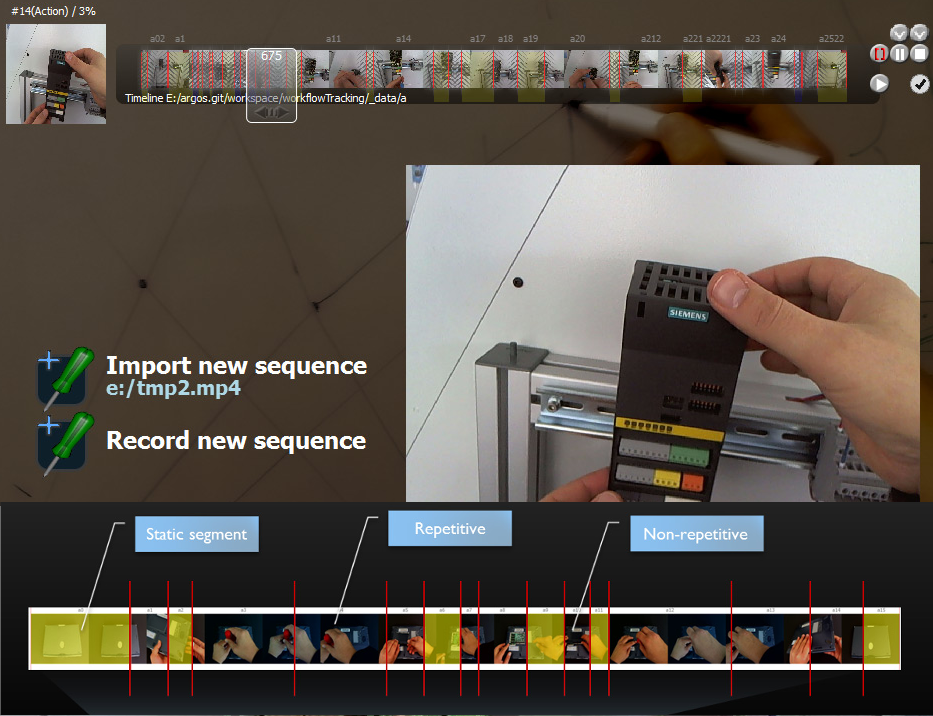
\includegraphics[width=0.8\textwidth]{img/ar-authoring.png}
  \caption{Authoring f�r das AR-Handbuch nach dem automatischen
  Vorverarbeitungsschritt, aus
  \cite{Niels2013}}
  \label{fig:ar-authoring}
\end{figure}
% ============================================= %

% ============================================= %
\begin{figure}[h]
\centering
\subfigure[]{
   	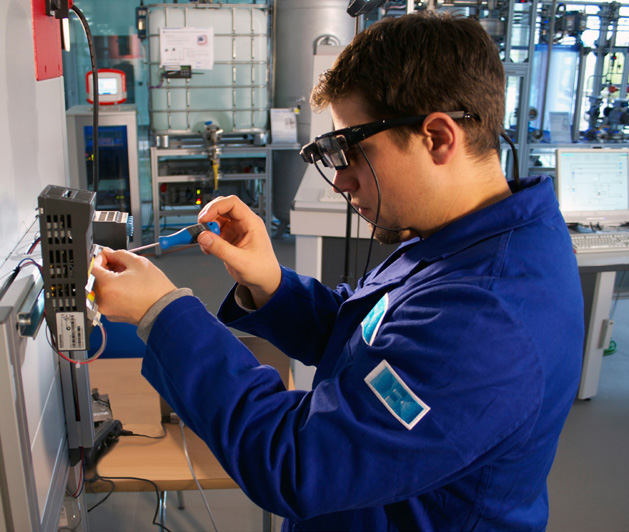
\includegraphics[scale=0.8]{img/ar-handbook-outside_view.png}
	\label{fig:ar-outside}
}
\subfigure[]{
   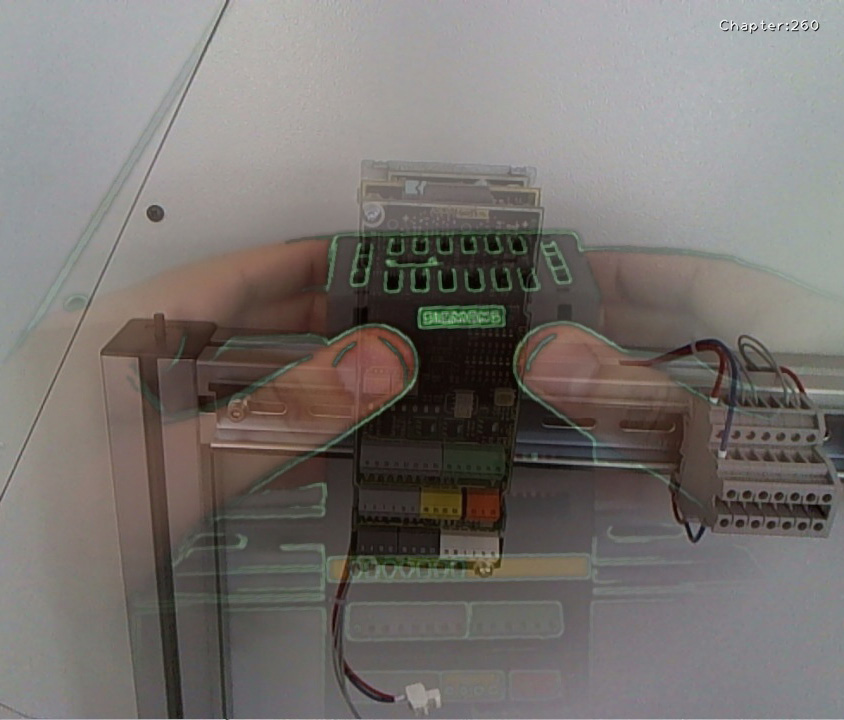
\includegraphics[scale=0.8]{img/ar-handbook-overlay_bsp.jpg}
   \label{fig:ar-overlay}
}
\subfigure[]{
   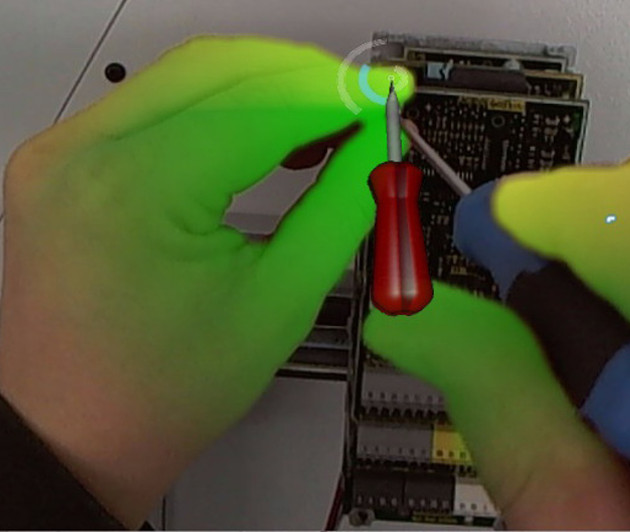
\includegraphics[scale=0.8]{img/ar-handbook-glove_green.jpg}
   \label{fig:ar-glove_green}
}
\caption{Das AR-Handbuch System aus \cite{Niels2013}}
\label{fig:}
\end{figure}
% ============================================= %

% =======
\subsection{Second-Sighted Glasses}
% =======

Ein zweiter Ansatz, auch auf AR basierend wird in \cite{Yone2011} vorgestellt.
Bei dem Second-Sighted Glasses Ansatz handelt es sich um die visuelle
Einblendung der verschiedenen M�glichkeiten, die ein Nutzer in der Interaktion
mit den Objekten, die ihn umgeben, hat.
Das Ziel ist es dem Benutzer zu zeigen mit welchen Aktionen bestimmte Ziele
erf�llen. Die m�glichen Varianten, auch \emph{Futures} genannt, werden abh�ngig
vom Kontext in dem sich der Benutzer befindet angezeigt.
Diese repr�sentieren m�gliche Abl�ufe die vom Kontextsensitiven Systemen
definiert werden. Objekte sind mit Hilfe von Markern mit einer vorher
definierten Aktion verbunden und l�sen eine Mixed-Reality Animation aus, wenn
sie in das Blickfeld des Anwenders kommen.
Laut den Autoren muss noch weitere Forschung betrieben werden, um die
automatische Generierung von Animationen aus den Kontextdefinitionen zu erlauben
und um die Zusammenarbeit mit anderen Kontextsensitiven Systemen zu erm�glichen.

AR-Technologien werden noch nicht in der breiten Masse angewendet. Aber
Zunehmend mehr Forschung in die Massentauglichkeit von AR-Brillen wird
durchgef�hrt. CastAR \cite{CastAR2013} zum Beispiel, ist ein AR-System, dass f�r
rund 200 US-Dollar demn�chst auf den Markt kommen soll.
Kosteng�nstige Hardware k�nnte es Ans�tzen wie in \cite{Niels2013} oder
\cite{Yone2011} erlauben sehr schnell in den Nutzermarkt einzusteigen und breite
Anwendung zu finden.


% Language \cite{Yone2009} entwickelt
% Um den Objekten der Umgebung Intelligenz zu verleihen werden Sensoren oder
% Marker angebracht, die es erm�glichen ein reales Objekt mit der virtuellen
% Beschreibung der m�glichen Interaktionen zu verbinden. Da der Kontext eines
% Objektes schwer zu definieren ist wurde die Smart Object Event Modeling
% Language \cite{Yone2009} entwickelt. Diese erlaubt es trotz ihrer Einfachheit
% die Lesbarkeit, Portabilit�t, Expressivit�t und die Unabh�ngigkeit zwischen
% Modell und Zielobjekt zu wahren. Temporale Folgen die komplexe Abl�ufe
% defieneiren k�nnen dargestellt werden.


% [Bild SecSighGlasses?]

%% SOEML
%% Cum integrez nu prea stiu .. usable as task description language?
% Install this before that? Wait ten seconds
% Take some more shit from robotics?
% This paper proposes a smart object event modeling language. By attaching sensor nodes to 
% everyday objects, users can augment the objects digitally and apply the objects into various 
% services.  When  creating  such  smart  object  services,  users  should  define  events,  such  as 
% beverage of a cup turns cold or someone sits down on a chair, using physical values from 
% sensors. The  most common event definition for end-users  is simply describing threshold of 
% sensor values and boolean operation. When they want to define more complex events, such as 
% multiple people sit down on chairs or a user starts to study using a pen and a notebook, they 
% need to use a programming language. To define such complex event easily without complex 
% programming language, we present a new event description language called SOEML based 
% on  temporal  relation  among  simple  events.  We  also  provide  users  a  visual  interface  to 
% support users defining or reusing events
%  easily. [\cite{Yone2009}?]

% Auch eine graphische Oberfl�che f�r die Modellierung von SOEML wird angeboten.

% Die Autoren identifizieren bei diesem Ansatz die Notwendigkeit eine
% Benutzerstudie durchzuf�hren, um zu kl�ren ob die Benutzer die smarte
% Umgebung gut genug verstehen k�nnen und ob die Installation von den
% Entwicklern gut durchgef�hrt werden kann.  Weitere Forschung muss noch
% betrieben werden um die Generierung von Animationen aus den
% Kontextdefinitionen zu erlauben und um die Zusammenarbeit mit anderen
% Kontextsensitiven Systemen zu erlauben.

%% ==================================================
%% Authoring of a Mixed Reality Assembly Instructor for Hierarchical Structures

%% Asta ar veni in addition to VR-Handbook
% \cite{Zauner2003}
% Benutzen Marker und Authoring Tools um die Inhalte zu generieren.
% They argue that Mixed Reality allows a smooth combination of the real and the
% virtual world. Thereby, the user doesn't have to make a logical connection
% between the physical world and the virtual description of the instructions,
% which would greatly hinder him/her.
% They also mention a tablet PC may be used for MR.
% They proposed a State diagram of the Mixed Reality Assembly Instruction which
% uses a stack. Elements are pushed on the stack if they are composed of other
% elements. After the base elements have been found and assembled they are poped
% from the stack.
% When the user has to find an element a 2D user interface is used, Our approach
% for this problem is to aug- ment reality with a small animation of the placement
% pro- cess.
% More detailed installlation instructions visually and via audio Hierarchicall
% component structure: Composed components, base components

%% Vor candva sa aplice tehnica si pe masiniarii industriale. 
% % ===========================
\section{Produktspezifische Dokumentengenerierung}
\label{sec:documentGeneration}
% % ===========================

Die Erstellung von Benutzeranleitungen f�r industrielle Anwendungen ist neben
der Komplexit�t der Systeme auch von ihrer Variabilit�t abh�ngig. Um die
Generierung von Dokumenten als auch von Softwaresystemen aus demselben
Variabilit�tsmodel zu erlauben, wird in \cite{Rabiser2010} ein Ansatz
vorgestellt, der die Generierung der Dokumente mit der Konfiguration des
eigentlichen Produktes steuert. Grundlegend bei der Konzipierung des Ansatzes
ist die Beobachtung, dass viele Entscheidungen die w�hrend der Ableitungsphase
des Produktes gemacht werden, sowohl f�r die Dokumentation als auch f�r das
Softwaresystem relevant sind.
Die technische Realisierung des Ansatzes besteht aus den \dopler Werkzeugen
\cite{Dhungana2007, Dhungana2010} und wurde erfolgreich auf zwei industriellen
Produktlinien angewandt.

% % =======
% \subsection{Flexibler Ansatz zur Dokumentengenerierung}
% \label{sec:doplerSchritte}
% % =======

Der in \cite{Rabiser2010} beschriebene Ansatz ist unabh�ngig vom Reifegrad, der
Variabilit�tsmodellierung oder den zu generierenden Dokumenttypen. Bei der
iterativen Durchf�hrung der folgenden Schritte, sind Dom�nenexperten stark
eingebungen.

\begin{enumerate}
  \item Extrahieren und Analysieren der Dom�nenvariabilit�t
  
  \item Variabilit�ts-Modelle erstellen oder anpassen
  
  \item Variabilit�ts-Mechanismus und passenden Generator erstellen
  
  \item Dokumente um Variabilit�ts-Information erweitern
\end{enumerate}

Durch die Extraktion der Dom�nenvariabilit�t durch Produktlinienexperten und
Dom�nenexperten des Produkt-Managements oder des Vertriebs kann der wesentliche
Teil der existierenden Variablit�t identifiziert werden (Schritt 1). Mit den so
gewonnenen Informationen ist es m�glich, Variabilit�tsmodelle zu erstellen oder
anzupassen (Schritt 2).
Die gew�hlte Modellierungstechnik sollte flexibel sein und fortgeschrittene
Automatisierung w�hrend der Produktableitung zulassen. Um
Variabilit�tsinformation in den Dokumenten abzulegen ben�tigt man einen
Mechanismus, wie zum Beispiel ein strukturiertes Dokumentenformat mit einer XML
basierten Markupsprache (DocBook) (Schritt 3). Diese Informationen werden von
einem Generator benutzt, um die produktspezifischen Dokumente zu erstellen
(Schritt 4).
  
% =======
\subsection{\dopler Metamodell}
% =======
% ============================================= %
Die Realisierung des Ansatzes ben�tigt ein Metamodell, dass zwei Grundlegende
Entit�ten definiert: \emph{Assets} und \emph{Decisions} (vgl. Abbildung
\ref{fig:dopler-meta_model}). Assets sind Artefakte der Produktlinie, wie
Dokumente oder Technische Komponenten. Decisions hingegen sind die
Entscheidungsbasis, anhand derer die Konfiguration der Assets stattfindet. Diese
sind analog zu den in der Variabilit�tsmodellierung eingesetzten
Entscheidungspunkten (Variation Points).\\
% ============================================= %
Die im Metamodell vorhandene Abh�ngigkeitsbeziehung zwischen Assets modelliert
die Funktionsabh�ngigkeit und den strukturellen Aufbau des Systems. Logische und
hierarchische Zusammenh�nge zwischen den zu treffenden Entscheidungen
(Decisions) werden im Metamodell ber�cksichtigt und erlauben die Definition von
Reihenfolge- und Verhaltensbeziehungen.
Die \dopler Werkzeuge sind in der Lage, Dom�nen, durch dom�nenspezifische
Metamodelle, mit beliebiger Granularit�t und Abh�ngigkeiten zu modellieren,
solange deren Elemente von den Grundentit�ten \emph{Asset} und \emph{Decision}
erben.

%=======
\begin{figure}[htb]
  \centering
  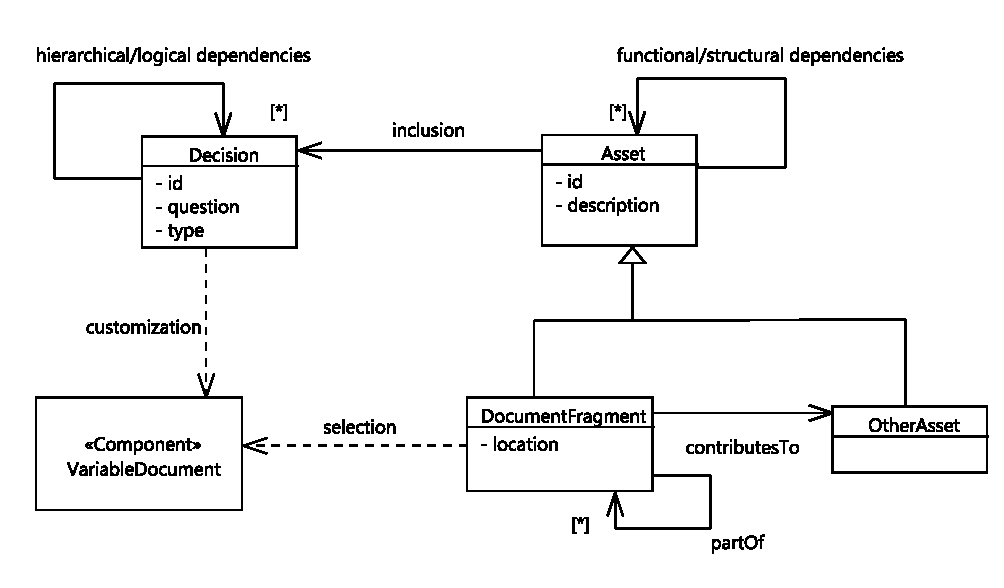
\includegraphics[width=0.8\textwidth]{img/dopler-meta_model_complete-me.pdf}
  \caption{\dopler\ Meta-Model mit Dokumenten aus \cite{Rabiser2010}.}
  \label{fig:dopler-meta_model}
\end{figure}
%=======

Die Inklusion eines Asset in das abgeleitete Produkt geschieht durch seine
Verbindung zu der Decision. Dom�nenexperten beantworten die zu der Decision
geh�rende Frage und instanzieeren dadurch die konkrete Konfiguration.
Durch diesen Mechanismus wird die Generierung der Dokumente gesteuert, indem ein
Dokumentenfragment ein Asset ist, dass zu anderen Systemkomponenten eine
Verbindung hat (siehe Abbildung \ref{fig:dopler-meta_model}). Ein
Dokumentenfragment repr�sentiert dabei Teile eines Dokumentes wie Kapitel oder
Abschnitte. Dokumentfragmente und Komponenten des Systems k�nnen dadurch
einheitlich behandelt werden. Dokumentfragmente erlauben die Modellierung der
grobk�rnigen Variabilit�t. Feink�rnige Anpassungen werden durch einen
spezifischen Variabilit�tsmechanismus realisiert.

% Auch die Attribute eines Asset k�nnen von den
% Antworten auf die Frage der Decision beinflusst werden. Die wesentlichen
% Elemente einer Decision sind die Frage und der Typ. Die Frage wird dem Nutzer
% bei der Konfiguration gestellt und dessen Antwort bestimmt die Zusammensetzung
% des Dokumentes, wobei der Typ das weitere Vorgehen bestimmt. Bei dem Typen der
% Decision werden von bin�ren Antworttypen (Ja/Nein Antworten) bis hin zu
% komplexer Logik darstellende Datentypen verwendet ([Beispiel ??]).


% \dopler erlaubt es dom�nenspezifische Assets zu definieren, indem ein vom
% \dopler Metamodell erbendendes Modell einer spezifischen Organisation oder
% Kontextes erstellt wird. Um Dokumente zu generieren kann man Teile oder sogar
% ganze Dokumente als Assets in den Modellen repr�sentieren. So wurden, wie in
% Abbildung \ref{fig:dopler-meta_model}, die Assets erweitert in dem das
% \emph{DocumentFragment} eingef�hrt wurde. Dieses kann Teile eines Dokumentes wie
% Kapitel oder Abschnitte repr�sentieren. Um auch den Fall zu modellieren, dass
% bestimmte Fragmente Teil von anderen Fragmenten sind, wurde in dem abgebildeten
% Modell eine Aggregation zwischen den Dokumentfragmenten eingef�hrt.

% =======
\subsection{\dopler Werkzeuge}
% =======

Die \dopler Werkzeuge benutzten den Profil-Mechanismus des
DocBook-Standards\footnote{www.docbook.org/}, um Elemente und Attribute zu
implementieren, die die Variationspunkte in den Dokumenten definieren.

% Die zentrale Erweiterung zu DocBook ist das \emph{doplerdoc} Attribut. Es
% koppelt das Markup-Element an ein Dokumentfragment und erlaubt es so optionale
% oder alternative Texte zu definieren.

Listing \ref{lst:dopler_docbook_xml} zeigt ein Beispiel aus einem
DocBook-Dokument mit der \dopler Erweiterung. Das Kapitel \emph{cooling} wird in
die Dokumentation nur aufgenommen, wenn das Dokumentfragment
\emph{cooling\_chapter} aufgrund einer Decision aufgenommen wurde.  Durch den
DocBook Mechanismus sind auch Querverweise m�glich und Platzhalter k�nnen in
Verbindung mit dem \emph{doplerdocplaceholder} Element erstellt werden.

% =======
\lstset{breaklines=true,language=XML,caption={Das Element
\emph{doplerdocplaceholder} mit dem \emph{doplerdoc} Attribut dient als
Platzhalter f�r den K�hlungsmechanismus \emph{cooling\_mech}
\cite{Rabiser2010}},label=lst:dopler_docbook_xml}
\lstinputlisting[language=XML]{listings/docbook_example.xml}
% =======

Der Ablauf zur Generierung von Dokumenten beginnt mit der Erstellung eines
Variabilit�tsmodells (Abbildung \ref{fig:dopler-process}). Die Antworten auf die
Fragen der Decisions werden durch den Nutzer mit Hilfe eines
Konfigurationsassitenten (z.B. \dopler Konfigurations-Wizard) in das Modell
eingetragen. Das variable Dokument, das zentrale Artefakt im Prozess der
Dokumentengenerierung, entsteht durch das Erweitern existierender Dokumentation
mit der im Variabilit�tsmodell existierenden Variabilit�tsinformation und eine
st�ndige R�ckkopplung zu dem Variabilit�tsmodell.

% =======
\begin{figure}[htb]
  \centering
  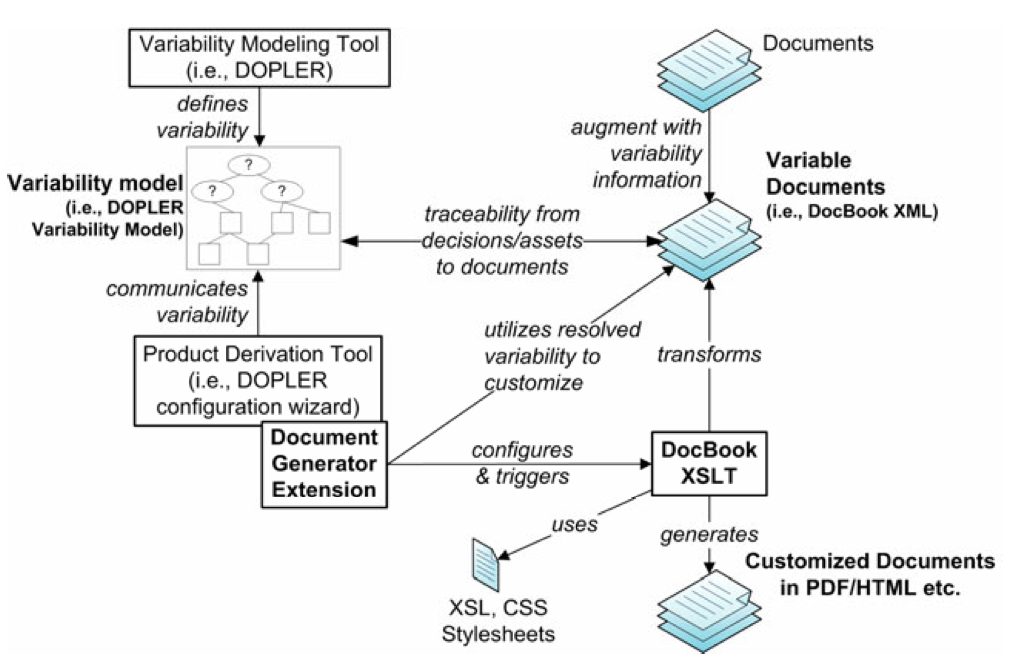
\includegraphics[width=0.8\textwidth]{img/dopler-document_generation.png}
  \caption{\dopler �berblick �ber den Generierungsprozess der finalen
  Dokumentation aus dem Variabilit�tsmodell in
  \cite{Rabiser2010}.}
  \label{fig:dopler-process}
\end{figure}
% =======

Der Dokumentengenerator passt mit Hilfe der aufgel�sten Variabilit�t das
Dokument-Template an und startet die DocBook-XSLT-Engine, um ein Dokument im
gew�nschten Ausgabeformat (z.B. PDF) zu erstellen. Formattierungsoptionen sind
mit XSL oder CSS realisiert und sind durch Decisions konfigurierbar.

% =======
\subsection{Industrielle Anwendung}
% =======

Die in den Studien aus \cite{Rabiser2007} eingesetzte Werkzeugkette, besteht
aus verschiedenen Auspr�gungen des \dopler Werkzeugs. Das \dopler
Variabilit�ts-Modellierungs-Tool und der \dopler Konfigurations-Wizard, der den
Nutzer durch die Produktableitung f�hrt, sind Teil davon. Als Generator dient
eine dom�nenspezifische Erweiterung des \dopler Konfigurationswerkzeugs.\\
% ============================================= %
Im ersten Anwendungsfall, bei der Siemens VAI, wurde auf einer schon
bestehenden, automatisierten Software-Entwicklungskette aufgebaut. Ein Gro�teil
der Decisions f�r die Dokumentengenerierung konnte aus den schon bestehenden
Variabilit�tsmodellen extrahiert werden. F�r den restlichen Teil sind
Dokumentenspezifische Decisions in Zusammenarbeit mit Dom�nenexperten erstellt
worden. Ein einziges Entscheidungsmodell steuert die Produktkonfiguration als
auch die Erstellung der technischen Benutzerdokumentation.\\
% ============================================= %
In der zweiten Industriellen Anwendung, bei der Siemens AG, mussten
kundenspezifische Verkaufsdokumenete erstellt werden, wobei es keine existierende
Variabilit�tsmodellierung gab. Zu den unten erw�hnten Variabilit�tspunkten kamen
noch variantenabh�ngige Berechnungen der Preise und anderer Indikatoren hinzu.
Au�erdem gab es in diesem Fall mehr Alternativtexte und einige Variationspunkte
die einen dokumenten�bergreifenden Einfluss hatten.

In beiden Anwendungsf�llen wurde mit Hilfe einer Befragung der Dom�nenexperten
die am h�ufigsten auftretende Variabilit�t in Dokumenten gesammelt:
\begin{itemize}
  \item Querverweise und deren Konsistenz
  \item Optionale Teile
  \item Platzhalter (z.B Name des Kunden)
  \item Grammatikalische Variation (Pluralbildung)
  \item Multi-Media-Objekte (z.B. Bilder)
  \item Formatierung und Layout (durch XSL oder CSS Style-Sheets
  realisierbar)
\end{itemize}

Der in \cite{Rabiser2010} beschriebene Ansatz erlaubt es an den Entwicklungs und
Generierungsprozesses von Software die Generierung von Dokumenten einzubinden.
Die Auswechselbarkeit der Werkzeuge zur Variabilit�tsmodellierung und
Generierung erlauben eine gro�e Flexibilit�t bei der Anwendung auf verschiedene
Dom�nen und unterschiedliche technische Gegebenheiten. Besonders
nicht-technisches Personal wird durch die so entstandene Werkzeugkette in der
Generierung von spezifischen Dokumenten unterst�tzt.

%Die beschreibung der Systemmodelle wird nicht erl�utert - vielleicht in anderen
%Papern? - Paper zu Eclipse

% Ein weiterer Aspekt ist der gro�e Konfigurations- und Interaktionsraum bei
% Anwendungen der Heimautomatisierung. Laut \cite{Pohl2005} ist die
% Heimautomatisierung eine Komplexe Anwendung, die dank der vielen Interaktions-
% und Konfigurationsm�glichkeiten einer Produktlinie �hnelt. Die Anpassung an
% den Kundenwunsch, verschiedene Kombinationen von Heimautomatisierungsprodukten
% (wie z.B. Heizungs-, Licht-, Fenstersteuerung o.�.) anzuschaffen, verk�rpert
% die Variabilit�t im Sinne von Produktlinien.
% Je nach Konfigurationswunsch sind diese verschiedenen Varianten des
% Heimautomatisierungsproduktes auszuliefern und in verschiedenen Arten zu
% installieren und zu warten. Der Kontext des Benutzers spielt dabei eine
% wesentliche Rolle. Der Vergleich zwischen der Heimautomatisierung und
% Produktlinien von \cite{Pohl2005} erlaubt es Prinzipien aus den
% Software-Produktlinien auf das Szenario der Heimautomatisierung anzuwenden.
% Rabiser et al. setzen f�r die Erstellung von produktspezifischer Dokumentation
% in der Industrie auf einen produktlienenbasierten Ansatz \cite{Rabiser2010}.
% Ein Generator erstellt das Dokument mit Hilfe des systemdefinierenden
% Variabilit�tsmodells. Die Kopplung von Software- und Hardware-Komponenten zu
% Teilen der Dokumentation erlaubt es die Konfiguration der Dokumentation
% zusammen mit der Systemkonfiguration durchzuf�hren. Der Ansatz basiert auf
% einer starken Einbeziehung der Dom�nenexperten und die zu den Komponenten
% geh�renden Textfragmente, m�ssen manuell mit dem eigentlichen
% Systemkomponenten synchronisiert werden.\\

% Bei der ersten Produktlinie handelt es sich um eine Anwendung zur
% Prozessautomatisierung von Siemens VAI, dessen technische Variabilit�t schon
% modelliert war und technische Dokumentation erstellt werden sollte. Die zweite
% Anwendung verlief bei der Siemens AG und es mussten ohne ein schon vorhandenes
% Variabilit�tsmodell kundenspezifische Verkaufsdokumente erstellt werden.

% \begin{figure}[htb]
%   \centering 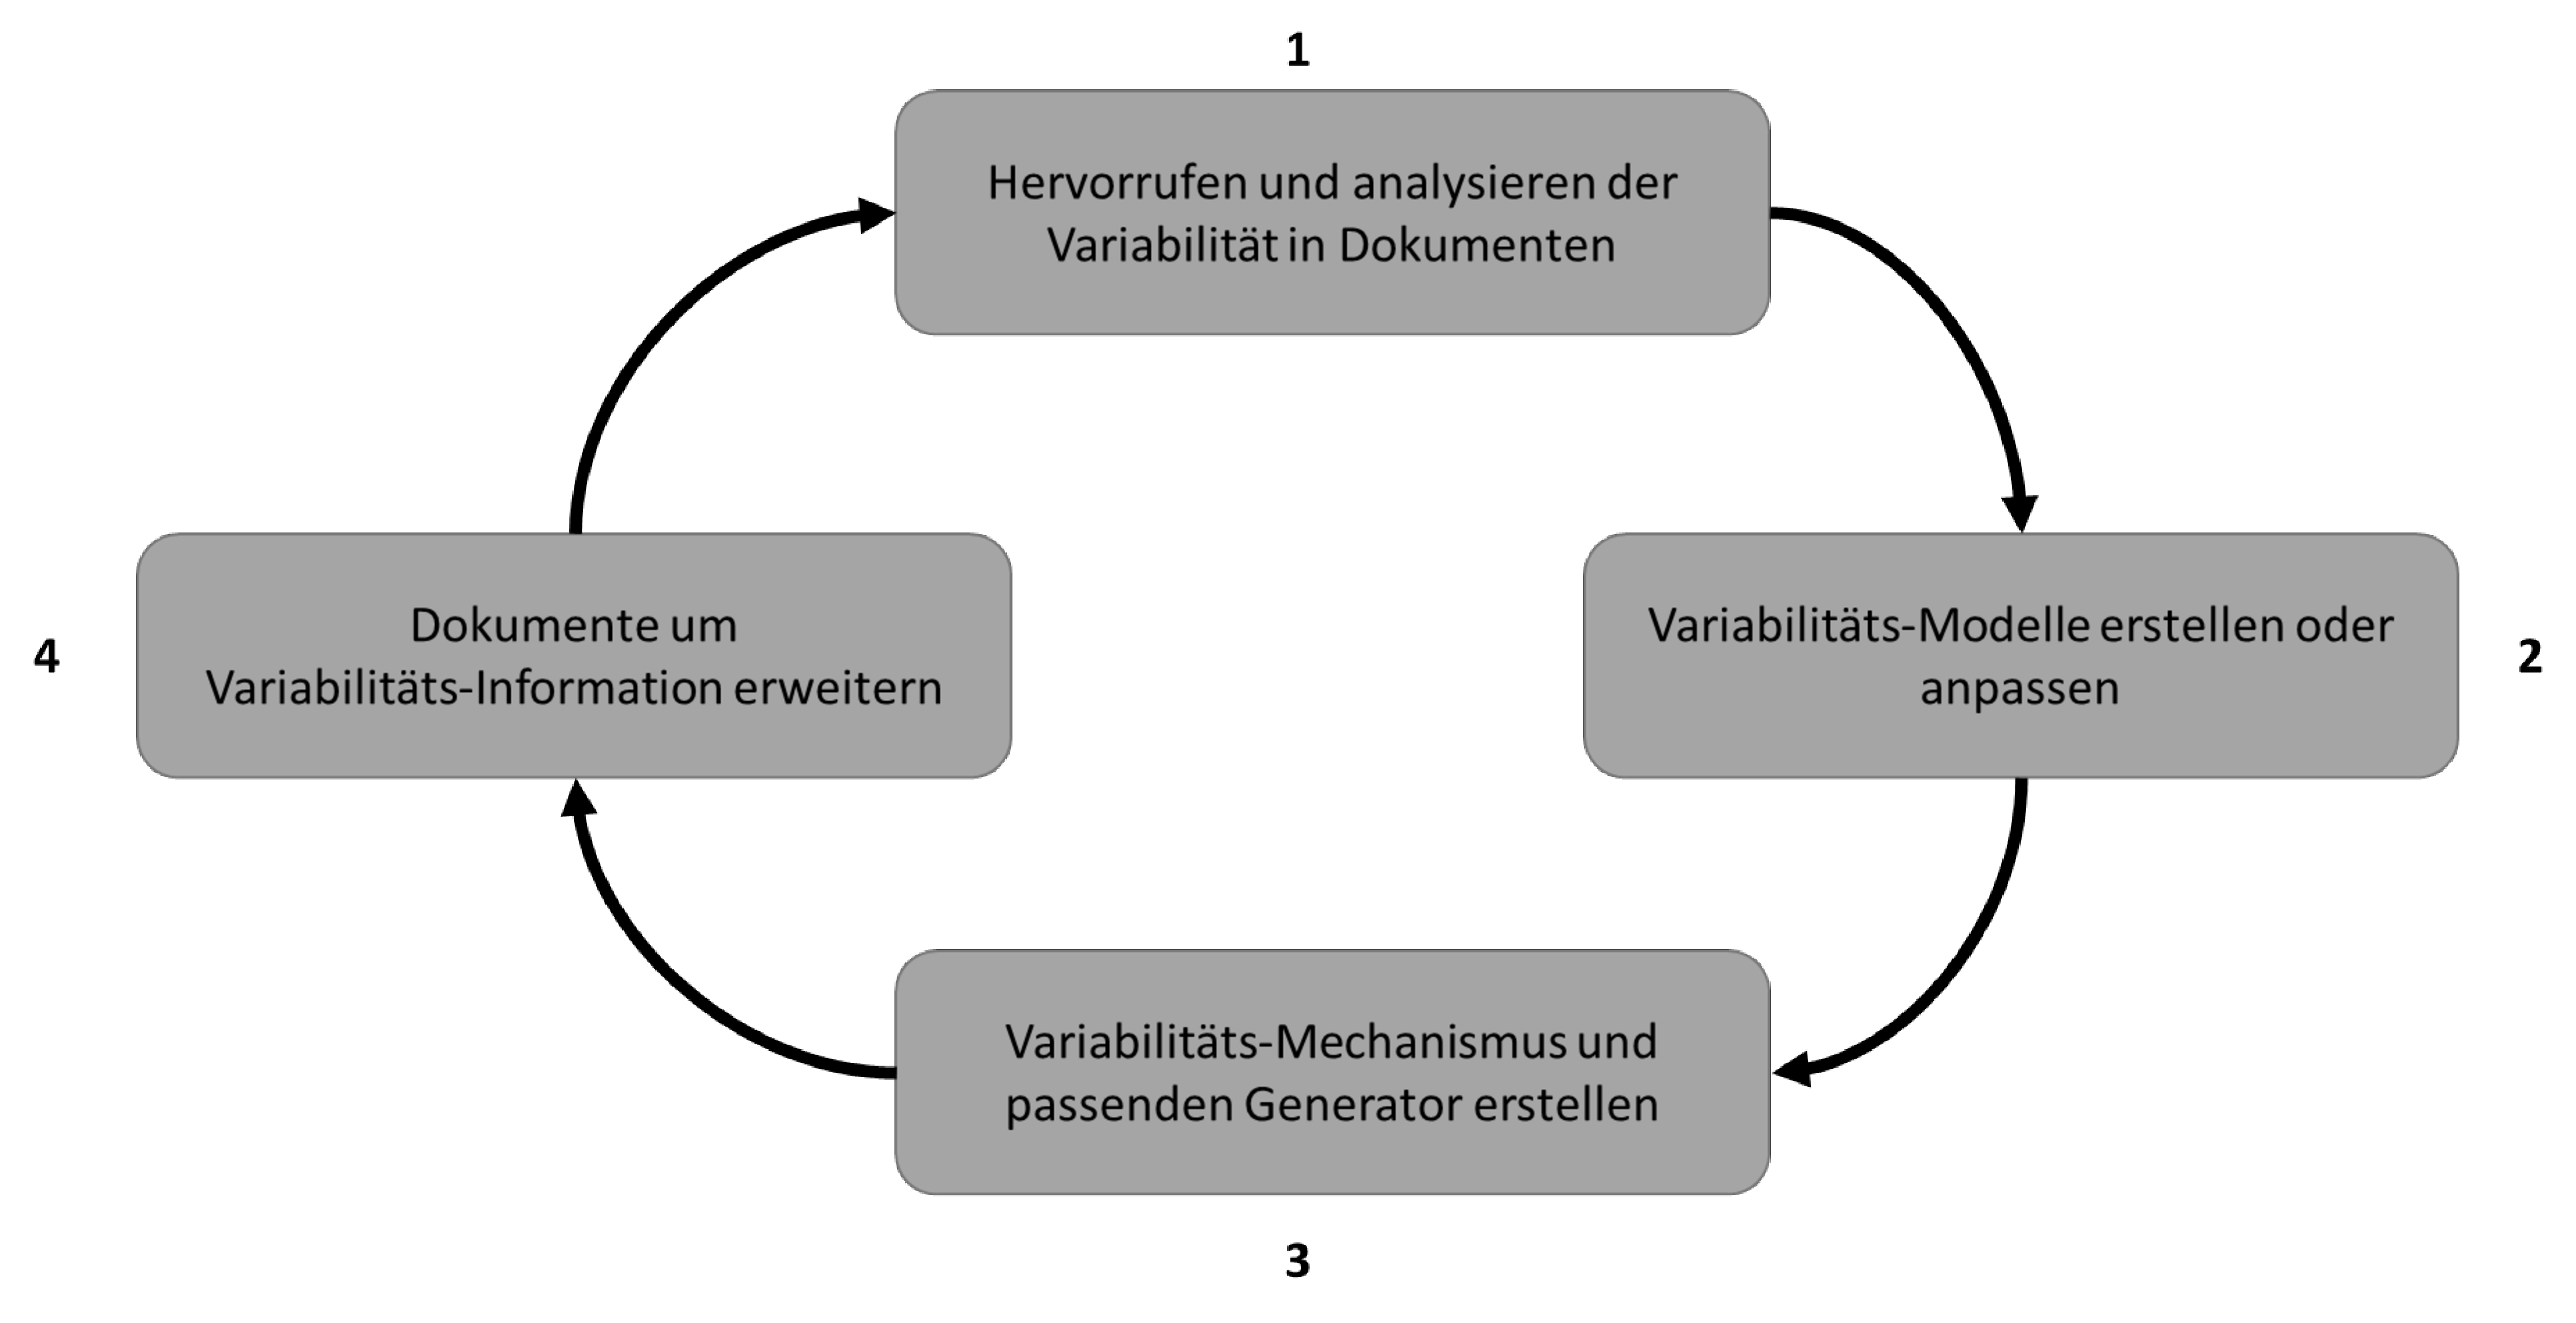
\includegraphics[width=0.9\textwidth]{img/dopler-approach.pdf}
%   \caption{Die vier iterativ zu durchlaufenden Phasen des Ansatzes zur
%   Dokumentengenerierung aus \cite{Rabiser2010}. Variationspunkte und Varianten
%   werden in Schritt (1) von Dom�nenexperten hervorgehoben und in Beziehung mit
%   den Modellen aus Schritt (2) gestellt. Die Beziehungen werden mit Hilfe des
%   Mechanismus aus Schritt (3) realisiert. Der letzte Schritt (4) webt die
%   Informationen in die Dokumente ein.}
%   \label{fig:dopler-approach}
% \end{figure}

% % nl_generation.tex %

%% ==============
% \section{Generierung von nat�rlicher Sprache aus Software-Modellen}
\section{Modellbasierte Erstellung von Dokumentation}
\label{ch:}
%% ==============

Der unterschied zw model driven und model based cu ref MDA ?

Die automatisierte Generierung aus den formalen Modellen eines Systems, umgeht
dieses Problem. Die systematische Literaturrecherche aus \cite{Nicolas2009}
analysiert automatisierte Ans�tze der Generierung von nat�rlichsprachlichen
Texten aus den formalen Modellen einer Anwendung. Die Autoren schlussfolgern,
dass das Thema in der Literatur schwach repr�sentiert ist, obwohl das Interesse
an dem Thema steigt und die Notwendigkeit solcher Ans�tze gegeben ist.
% % ============== 2009 SLR On the generation of requirements specifications
% from software engineering Models

%% ==============
\subsection{Literate Modeling}
\label{ch:sec:literate-modeling}
%% ==============
Inlocuiesti cu limone \cite{Schulze2012}
In this paper, we have presented an approach to address a major problem in
Literate Modeling: consistency between model and text. 
our approach attempts to provide fne-grained synchronization of
sentences in natural language with parts of the UML model.
 using text annota-
tions and a synchronization algorithm that uses natural language processing in
conjunction with OCL.
Feingranulare, per Satz Synchronisation


Explici putin ce ii cu literate modelling si apoi ca la topcased ce ii, la ce
se folosete, cum functioneaza, cum e realizat?
% Limone? da nu stiu cat de mult pot spune despre el\ldots 
Unter \emph{Literate Modeling} versteht man die von \cite{Arlow1999} eingef�hrte
Methode, in der das Anforderungsdokument Systemmodelle zusammen mit narativem
Text vorsieht, um ein Gesamtbild des zu entwickelnden Systems zu geben.
Das so entstandene Dokument, auch \emph{Business Context Document (BCD)}
genannt, beinhaltet neben dem visuellen Modell auch nat�rlichsprachliche
Beschreibungen der UML Syntax, den Gedankengang der zu Entscheidungen f�hrte,
Beispiele zur Illustration bestimmter Aspekte und eine Umschreibung in
nat�rlicher Sprache des Modells.

Auch \cite{Burden2011} identifizieren dieses Probleme und benutzen einen
Ansatz, der �hnlicherweise grammatikalische Regeln als Unterst�tzung f�r die
Generierung anwenden.

Die Autoren arbeiteten zur Zeit der Entwicklung dieser Methode bei British
Airways. W�hrend der Systementwicklung trat ein Problem, dass die Autoren als
\emph{'trivialisation of business requirements by visual modelling'} nannten,
auf. Die Autoren haben beobachtet, dass nach der Formalisierung der
Anforderungen wichtige Kernaspekte der Dom�ne zwischen anderen unwichtigeren
Details untergehen. Ein Beispiel dieses Problems ist das Cross-Selling von
Flugtickets zwischen British Airways und den Allianzpartnern, ein Markt der
Ums�tze in Millionenh�he t�tigt und somit sehr wichtig f�r das Gesch�ft ist.
Diese Gesch�ftsanforderung wurde in dem UML Modell, korrekterweise, durch eine
mit dem * Symbol dargestellte Multiplizit�t an dem Assoziationsende zwischen den
Modellklassen Flug und Flugnummer dargestellt (vgl. Abbildung
\ref{fig:articulate-model}. Dadurch verlor diese Anforderung an Bedeutung bei
der Darstellung im formalen Modell. Nach der Einf�hrung von BCD konnten die
Gesch�ftsanforderungen enger an die Formalen Modelle gekoppelt werden und in
\cite{Arlow1999} wird berichtet, dass die Anwendung der Literate-Programming
Methode zu einer Verbesserung in der Umsetzung der Projekte gef�hrt hat.

Um diese Methode effizient zu nutzen, so merken die Autoren in \cite{Arlow1999}
an, wird eine gute Werkzeugunterst�tzung ben�tigt, die die Konstistenz zwischen
Modellen und dem beschreibenden Text gew�hrleistet. Aus diesem Grund wurde in
\cite{Schulze2012} ein Ansatz entwickelt, um die Synchronisation zwischen den
Diagrammelement und den Ihnen Beschreibenden nat�rlichsprachlichen Texten
durchzuf�hren. Der dort beschriebene Ansatz basiert auf die Annotierung des
Textes und einem Synchronisationsalgorithmus, der nat�rliche Sprache in
Verbindung mit OCL Ausdr�cken verarbeitet. Um den Ansatz prototypisch zu testen
wurde das Tool LiMonE\footnote{LiMonE:
http://squam.info/limone}, als Adapter f�r die Eclipse UML2 Tools und den
Papyrus Editor, in einer Masterarbeit, entwickelt.

% Besonders der Ansatz des Literate Modeling (vgl.
% \ref{ch:sec:literate-modeling}) wird in verschiedenen Arbeiten verfolgt.

The Business Context Document closes the comprehensibility gap between
the modeler and their non-technical audience and allows for effective review and
feedback on the models by non-technical stakeholders.

For synchronization of individual elements, we use text annotations that provide
the semantic link between a particular word of a sentence and the corresponding
element of the UML model

 Each annotation contains the unique resource identiffer
(URI) of the model element, as well as the fully qualifed name of the element
within the model

To take account of the modelfs structural features, sentences that contain refer-
ences to model elements need to be validated. This is achieved by checking each
sentence using a set of validation constraints. 

 For analyzing the structure of each sentence, we have
used the Stanford PCFG Parser 

Based on this representation, we have developed a language that allows us to
search for specifc grammatical relationships between individual constituents of a
sentence, as well as specify the type of the UML model elements particular words
have to be associated with. 

Internally, the sentence constraints are translated into an equivalent Prolog
query and evaluated using a light-weight Prolog system for Java

For expressing the second component of the validation
constraint, we use the Object Constraint Language (OCL) [17]. Validation con-
straints are required to work with all possible user models, hence we use OCL on
the UML metamodel layer (M2) to constrain elements of the user model (M1).
More precisely, the invariant mechanism of OCL is used to check whether a set
of classes conforms to certain structural requirements.

The presented approach has been implemented in a prototypic editor for Lit-
erate Modeling, called LiMonE 2 , which was used to conduct the experiments
discussed above. The tool has been developed as a plugin for Eclipse, and is
designed to interoperate with different modeling tools built on top of the
Eclipse platform. Currently, adapters for the Papyrus UML Modeler and the UML2
Tools of Eclipse are provided.
The editor allows the user to create a Business Context Document for a par-
ticular model, and embed the diagrams of the model in the document. Model
elements can be inserted via an auto-completion feature, which allows the user to
select from a list of suggested items. UML model and text can be edited simulta-
neously, with changes to individual model elements being updated immediately
in the Business Context Document. In case structural changes have been made
to the model, those sentences containing text annotations are validated after the
model or the text document have been saved. As already mentioned in section
3.2, changes can be detected even when the model is edited without the editor
being open. A list with the detected inconsistencies is shown in a separate view,
with the corresponding sentences being underlined in the editor.

Diagrams from the model can be added



\begin{figure}[htp]
\begin{center}
  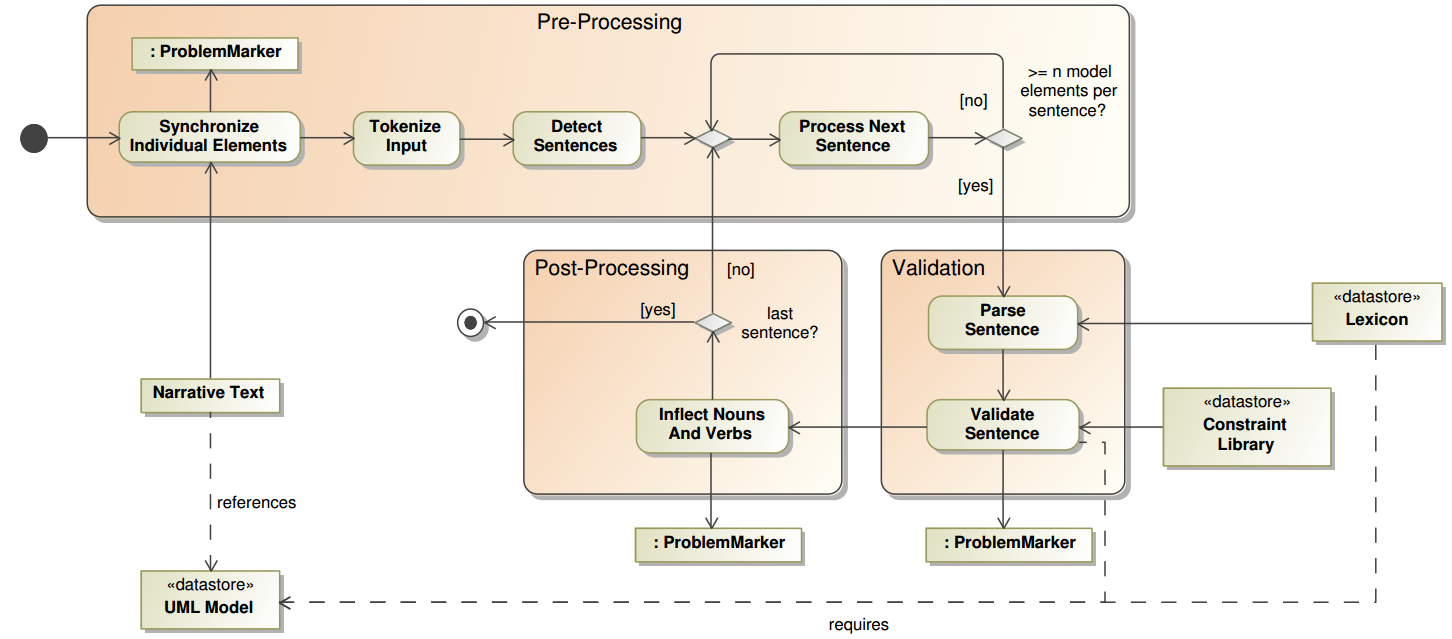
\includegraphics[width=0.8\textwidth]{img/limone-syncprocess.png}
  \caption[XX]{\cite{Schulze2012}}
  \label{fig:m2n-architecture}
\end{center}
\end{figure}
% 
% %% ==============
% \subsection{Articulate Modelling}
% \label{ch:sec:}
% %% ==============
% 
% %% xtUML einf�hren
% 
% [aus Buch Starr2001]
% Articulate modelling einf�hren (+xtUML) und sagen, dass das ein guter
% schritt ist um die Systembeschreibung zu verbessern und die NL
% generierung zu erleichtern. Dadurch entseht auch ein besserer Bezug
% zwischen den Modellen und Korrekturen k�nnen leichter in das
% Formale Systemmodell �bernommen werden.
%  What I am defining as an ''articulate'' class model is one
% that expresses critical system rules with transparent, unambiguous precision.
% 
% % The model should express the application's true require-
% % ments, as minimally and precisely as possible without telling the programmer how to write code.
% % 
% % DEFINING A PLATFORM INDEPENDENT CLASS
% % WHAT QUESTIONS CAN THIS CLASS ANSWER?
% % 
% % ENFORCING THE IDENTITY CONSTRAINT
% % 
% % RELATIONSHIPS
% % All relationships in the Good Model are glued together with referential
% % attributes. % asta nu prea am inteles
% % 
% % VERB Pharases
% % In fact, since the role name often matches the associated class name, you can usually drop them alto-
% % gether without affecting a model's expressiveness.
% % 
% % To read an association named using verb phrases, start on one side of the association and read the
% % phrase, multiplicity and class name on the opposite side as shown.
% % 
% % Main Idea: does the model express all the business rules? AND
% % Behavioral constraints satisfied? Can you answers certain questions of
% % situations that might arise during runtime?
% % 
% % Generic, all-inclusive verb phrases such as ''contains'', ''is a group of'',
% % ''has'' and my favorite  ''is associated with'' are to be avoided.
% 
% 
% 
% %% In diskussion: aus dem Articulate ding kann man die Verbphrasen nehmen, da
% % diese Unabh�ngig vom Tool das Benutzt wird erstellt werden k�nnen.
% 
% 
% % % 2011 Natural Language Generation from Class Diagrams
% % Burden hat auch Grammar dings gemacht mit Grammatical Framework,
% % ein..
% \begin{figure}[htp]
% \begin{center}
%   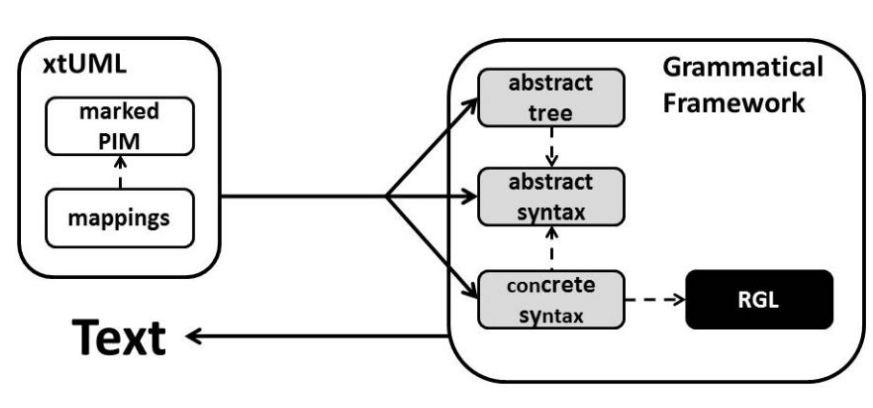
\includegraphics[width=0.6\textwidth]{img/burden-approach.png}
%   \caption[Ansatz aus \cite{Burden2011}]{}
%   \label{fig:burden-approach}
% \end{center}
% \end{figure}

Die Problematik der Interpretation von Formalen Modellen wurde auch in
\cite{Burden2011} behandelt. Klassendiagramme, die dem
Plattformunabh�ngigen Modell angeh�ren, wurden mit Hilfe des
Grammatical Framework (GF) \footnote{Grammatical Framework, ist eine
Anwendung f�r multilinguale Grammatikalische Anwendungen:
http://www.grammaticalframework.org/} in nat�rlichsprachige Texte
transformiert mit dem Zweck den Stakeholdern das
Verst�ndniss des Modells zu erlauben. Die Autoren sehen dies als wichtigen
Schritt um die korrekte �bersetzung der Anforderungsspezifikation in Form eines
CIM in das Software-Technische PIM zu �berpr�fen. Eine Validierung des
plattformunabh�ngigen Modells kann so durch Dom�nenexperten erfolgen und
eventuelle Fehler aus falsch verstandenen Als Nebeneffekt entdecken die Autoren
das Dom�nenexperten auch Fehler in den Originaldokumenten der
Anforderungsspezifikation gefunden werden, da die Repr�sentation als Formales
Modell  .. gehalten werden muss. Somit sind auch die daraus generierten Texte
frei von unklarheiten. Auch in \cite{Starr2001} wird erw�hnt, dass durch die
Verbphrasen an den Assoziationsenden viel �fter Fehler in den Modellen endeckt
werden.
% 
% Der Ansatz benutzt.. In Abbildung
% \ref{fig:burden-approach}..
% 
% 
% zu erlauben damit so die
% Transfomation vom CIM in das PIM validiert.
% Generalisierungsbeziehungen werden nicht erw�hntw
% 

\begin{figure}[htp]
\begin{center}
  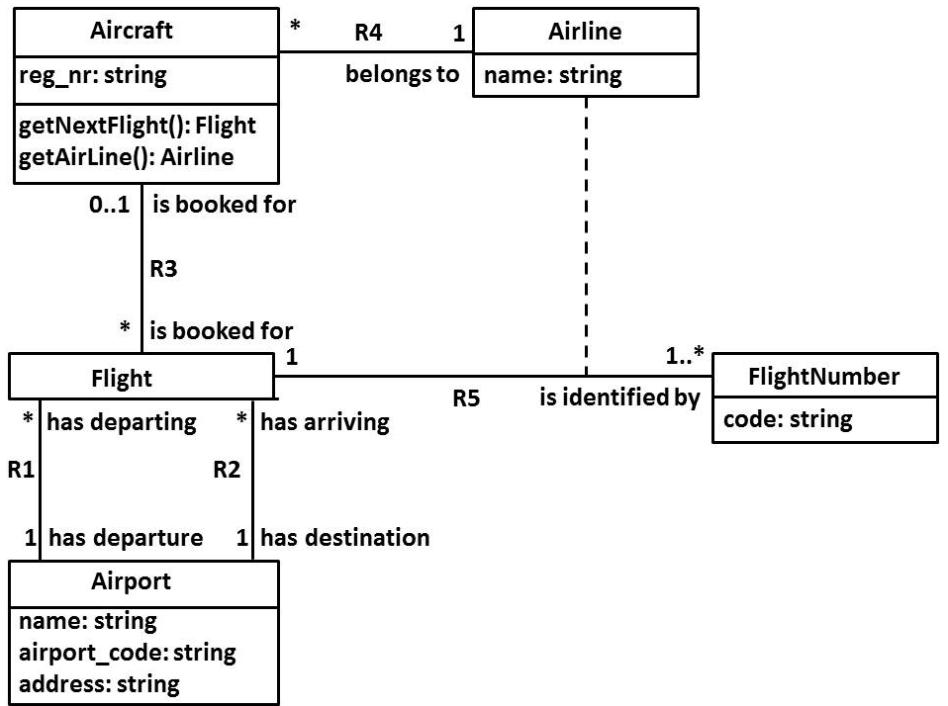
\includegraphics[width=0.8\textwidth]{img/airline-articulatemodel.png}
  \caption[Articulate Model, das Airline-Model]{Articulate Model aus
  \cite{Burden2011}. Die Verbphrasen and den
  Assoziationsenden erleichtern das Verst�ndnis beim Lesen des
  Modells}
  \label{fig:articulate-model}
\end{center}
\end{figure}

Im Folgenden wird ein Teil durch der in \cite{Burden2011}
pr�sentierten Technik erstellten Textes aufgef�hrt:

\begin{quotation}
\emph{An Airport has a name, an airport code and an address. An Aircraft can
get next Flight and get Airline. A Flight is identified by one or more
Flight Numbers. The relationship between a Flight and a Flight Number
is specified by an Airline. A Flight can have more than one Flight
number since code sharing is a multimillion-pound business, affecting
an alliance of airlines.}
\end{quotation}

Der Text orientiert sich sehr stark an das Diagramm aus
\ref{fig:articulate-model}, ist aber verst�ndlicher f�r Personen die nicht mit UML vertraut sind. Im
letzten Satz wurde auch das der Flight-Klasse angeh�ngte Kommentar
eingeflegt. Dadurch wird die Wichtigkeit der modellierten
Anforderung hervorgehoben.

% %% ==============
% \subsection{Template-basierte Generierung}
% \label{ch:sec:}
% %% ==============
% 
% 
% % % 2010 Position Paper m2n - A Tool for Translating Models to NL
% Anstatt eine Grammatik zu verwenden, wurde in dem in \cite{Brosch2010}
% pr�sentierten System, ein Ansatz entwickelt mit dem Textuelle Spezifikationen
% aus einem UML Klassen-Modell mit Hilfe von Satz-Templates erstellt werden. Die
% Autoren zielen mit dem Ansatz auf p�dagogische Anwendungsszenarien wie
% e-Learning oder �bungsbetrieb. Ein interessanter Beitrag dieser Arbeit ist, dass
% auch �berlegungen gemacht �ber die Traversierungsstrategie der Klassenmodelle
% wurden. Das wichtigste Element im Modell wird mit Hilfe eine Heuristik bestimmt,
% die Assoziationen und Generalisierungen auswertet, um von dort aus mit einer
% Tiefensuche das Diagramm zu bearbeiten.
 
%  
%  ODT or DOCX documents are XML archives
% Gendoc2 uses Model2Text (M2T) transformation language Acceleo
% Styles, formatting, structure and static content of the document are kept during 
% generation.
% \begin{figure}[htp]
% \begin{center}
%   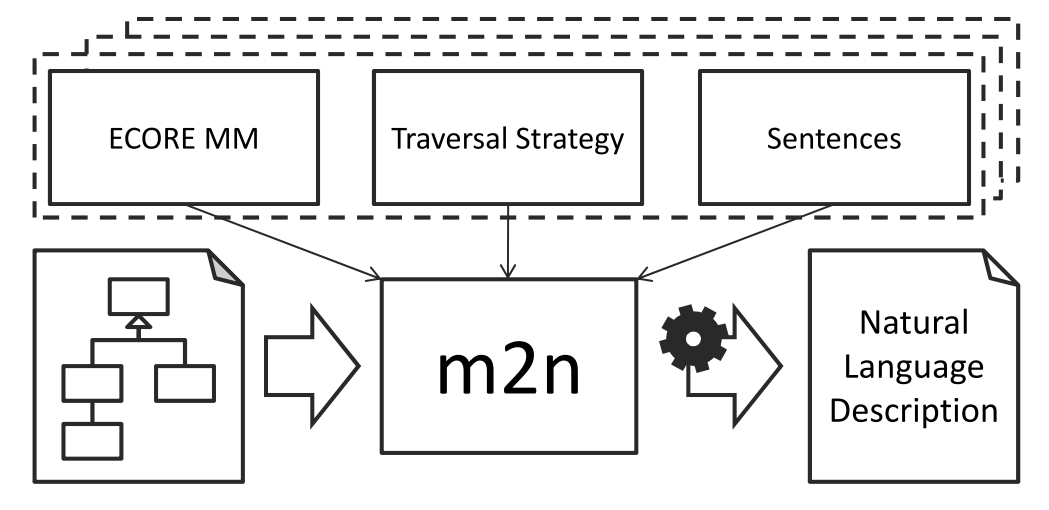
\includegraphics[width=0.9\textwidth]{img/m2n-architecture.png}
%   \caption[Das Tool m2n, Architektur]{Architektur des Tools m2n aus
%   \cite{Brosch2010}}
%   \label{fig:m2n-architecture}
% \end{center}
% \end{figure}
% 
% In \cite{Nicolas2009} werden weiter Ans�tze beschrieben die hier nicht
% erw�hnt werden, weil sie von bestimmten Tools abh�ngen und diese
% Arbeit einen leichtgewichtigen Ansatz sucht, der die Aufgabe der
% Generierung von Texten �bernehmen kann. Die Implementierung eines
% Prototyps, zur Generierung von nat�rlicher Sprache aus
% Software-Modellen, basierend auf den hier vorgestellten Ans�tzen
% sollte m�glich sein.
	

%% ==============
\section{Modellgetriebene Generierung von Dokumentation}
\label{ch:sec:}
%% ==============

Was ist topcased?
Wozu wird es benutzt/Wozu wurde es gebaut?

\cite{Pontisso06}

Modellierung standardisiert OMG MDA, graduelle verfeinerung
Anstrengungen der MDA si

MDSD an diesem Beispiel kurz erkl�ren

[Einleitung] Ein weiteres Werzkeug zur automatischen Generierung von
Dokumentation ist das in der Topcased Plattform enthaltene Gendoc, das aus
Quellmodellen modellgetriebene Erstellung von Dokumentation erm�glicht.

Topcased\footnote{http://www.topcased.org/ ab 2014 auf http://polarsys.org/} ist
ein Open-Source Werkzeug f�r modellgetriebene Entwicklung und dient dem System-
und Software-Engineering von kritischen und embedded Anwendungen. Die Plattform
unterst�tzt alle Entwicklungsstufen von der Anforderungsanalyse bis zu der
Implementierung. Sie basiert auf der Eclipse Plattform und benutzt das Eclipse
Modeling Framework (EMF), um einen modellgetriebenen Arbeitsfluss zu
realisieren. Es unterst�tzt neben UML Modellen auch andere von der OMG
standardisierten Modellierungssprachen wie SysML\footnote{http://www.sysml.org/} und
ReqIF\footnote{http://www.omg.org/spec/ReqIF/}.

Als Teil der Topcased Plattform erlaubt Gendoc die Generierung von textueller
Dokumentation aus UML Modellen. Die Generierung wird von Skripten in den
Dokumenten-Templates, die Logik und Modellabfragen beinhalten, gesteuert. Um die
Modellabfrage zu realisieren sind Acceleo Skripte und OCL Ausdr�cke m�glich.

Acceleo\footnote{} Skripte, die direkt in den Dokumenten-Templates geschrieben
werden lesen die Quelldomodelle mit Hilfe von OCL aus und f�llen das Dokument.
Die benutzten Skripte, die in der Acceleo Sprache geschrieben sind, k�nnen
beliebig Komplexe OCL Ausdr�cke wie Schleifen oder Logik enthalten. 

Topcased unterst�tzt einen Gro�teil der UML Modelle, namentlich sind das
Klassen-, Komponenten- und Deployment-Diagrammes, die die Struktur beschreiben
und Sequenz-, Aktivit�ts- und Zustandsdiagramme die die dynamischen Teile eines
Systems beschreiben. Auch Use-Case Diagramme k�nnen modelliert, abgefragen und
in die Dokumentation mit eingebunden werden.

Der generative Ansatz verl�uft wie in Abbildung \ref{fig:topcased-gendocflow}
dargestellt. Die Modelle und die Dokumenten-Templates sind die Eingaben des
Systems, als Ausgabe liefert Gendoc das ausgef�llte Dokumenten-Template. Die
Abspeicherung der ODT\footnote{} und DOCX\footnote{} Formate als XML, erlaubt es
Gendoc die Skripte zu extrahieren und Auszuwerten. Da die Skripte in der
Modelltransformationssprache Acceleo geschrieben sind k�nnen direkt auf die
Modelle ausgef�hrt werden. Dieser Ansatz erlaubt es, alle von der EMF
unterst�tzten Modellformate in Gendoc einzusetzen.

UML Modelle liefern Informationen �ber den erw�nschten Einsatz des Systems und
werden prim�r in Zusammenarbeit mit Dom�nenrepr�sentaten erstellt.

Die Skripte sind in einer Markup-�hnlichen Sprache eingebettet, die durch  und
HTML �hnliche Unterst�tzung von Bildern und Listen besitzen. 

Beim Auswerten der Skripte behalten die Ausgaben die Formattierung bei.
Graphische Elemente, wie konkrete Diagramme k�nnen aus dem
Quellmodell generiert werden und neben dem Text in das generierte Dokument
eingef�gt werden.
Da die Formattierung des Dokuments beibehalten wird ist die dynamische
Verlinkung mithilfe der Dokumenteneigenen Mechanismen m�glich.

Gendoc Befehlen werden durch das <gendoc> tag gekennzeichnet. Neben dem Acceleo
Skript sind auch statische Texte mit Formatierungen, Bilder und Tabellen
Erlaubt.

Hyperlinking ist m�glich durch das Benutzen des Dokumentformat abh�ngigen
Verlinkungsmechanismus.

Die Konfiguration, die die Erstellung des Dokumentes steuert wird auch im
Dokument-Template unter einem Markup-Tag gespeichert.

Ein Mechanismus zur Wiederverwendung von Code in den Templates steht zur
Verf�gung.

Zugriff auf alle Elemente der Diagramme die benutzt weredn um das System zu
modellieren. Volle Kontrolle auf die Erstellung des Dokumentes und der
Informationen die aus den Modellen abgeleitet werden.

Kann es andere Fragmente mit einbeziehen? Sind Acceleo Skript und Dokument immer
gemischt. Dom�nenexperten k�nnen dann wahrscheinlich nicht damit arbeiten.

Sagen dass Topcased auch code generieren Kann

Gendoc erlaubt es auch im Batch-Modus zu laufen, um automatisierte
Werkzeugketten zu realisieren.

Nachteil: Code aus Templates kann nur mit gro�em Aufwand auf ein Anderes
Template angewandt werden.

\begin{figure}[htp]
\begin{center}
  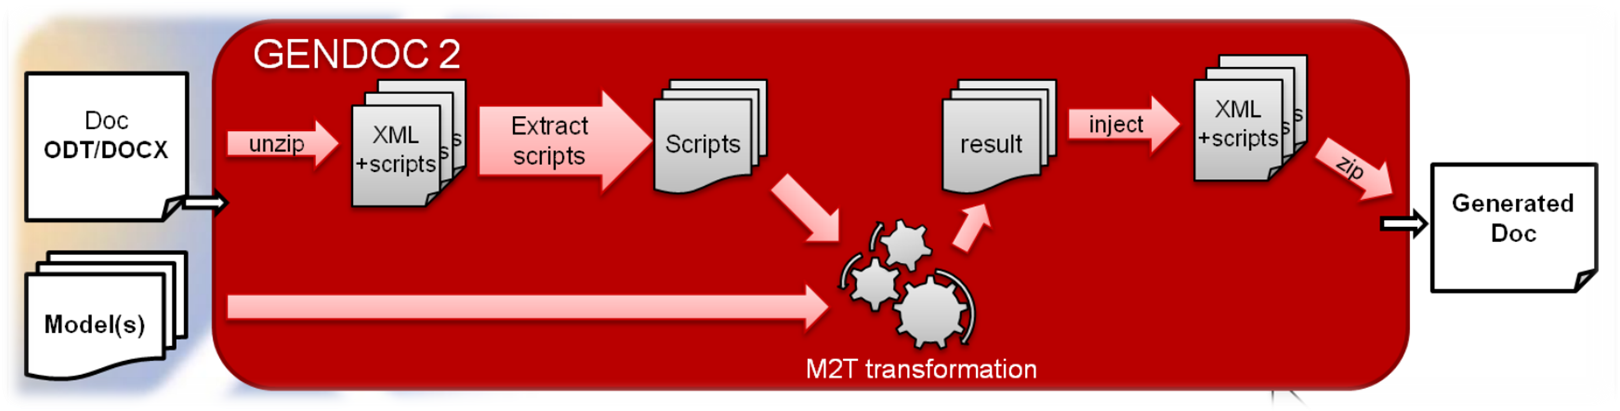
\includegraphics[width=0.6\textwidth]{img/topcased-gendocflow.png}
  \caption[XXX]{XXXXXXX}
  \label{fig:topcased-gendocflow}
\end{center}
\end{figure}


Wie funktioniert es?
	Konzeptuell
	Technische realisierung

	
% Listing erkl�ren was die einzelnen tags machen. Are rost listingu? Vezi daca se
% merita la dopler.
% % =======
% \lstset{breaklines=true,language=XML,caption={Das Element
% \emph{doplerdocplaceholder} mit dem \emph{doplerdoc} Attribut dient als
% Platzhalter f�r den K�hlungsmechanismus \emph{cooling\_mech}
% \cite{Rabiser2010}},label=lst:dopler_docbook_xml}
% \lstinputlisting[language=XML]{listings/topcased.xml}
% % =======

